\documentclass[conference]{IEEEtran}
\IEEEoverridecommandlockouts
% The preceding line is only needed to identify funding in the first footnote. If that is unneeded, please comment it out.
\usepackage{cite}
\usepackage{amsmath,amssymb,amsfonts}
\usepackage{algorithmic}
\usepackage{graphicx}
\usepackage{textcomp}
\usepackage{xcolor}
\usepackage{subcaption}
\usepackage{graphicx}
\def\BibTeX{{\rm B\kern-.05em{\sc i\kern-.025em b}\kern-.08em
    T\kern-.1667em\lower.7ex\hbox{E}\kern-.125emX}}
\begin{document}

\title{Deep Reinforcement Learning-Based Energy Trading of Microgrid with Mitigating the risk of disturbances 
\thanks{This is for the final report in ME 597: Distributed Energy Resources - Spring 2024 }
}

\author{\IEEEauthorblockN{1\textsuperscript{st} Jae Heo}
\IEEEauthorblockA{\textit{School of Construction Management Technology} \\
\textit{Purdue University}\\
West Lafayette, IN, USA, 47906 \\
heo27@purdue.edu}

}

\maketitle

\begin{abstract}
The occurrence of large-scale disturbances has been increasing over 20 years in the United States. As a consequence of this trend, a primary concern of today's power system is to enhance its resilience. As an innovative solution, microgrids suggest an immense promising approach toward achieving a higher level of distribution system resilience by integrating with electricity load. Although previous studies have focused on maximizing the total prioritized load to be picked up, using mathematical programming and iterative algorithms, their model cannot be fully utilized into comprehensive situations with mitigating the load unbalance and capturing the uncertainty situation in the microgrid operation model, simultaneously. Thus, this project aims to detect emergency situation and mitigate the risk of load disturbance in energy trading using deep reinforcement learning. In particular, it can take optimal actions of detecting the emergency situation and minimizing the risk of disturbance in the energy trading. The results show that the proposed network model achieves a stable energy trading model under mitigation of the risk of disturbance. Thus, this study may help to identify the emergency situation in energy generation and consumption and mitigate the risk of disturbance in energy trading. 
\end{abstract}

\begin{IEEEkeywords}
Microgrid, Resilience, Large disturbance, Energy trading, Deep reinforcement learning
\end{IEEEkeywords}

\section{Introduction}
The escalating frequency and intensity of extreme weather events pose significant threats to energy infrastructures, with the electrical power system being particularly vulnerable to disruptions and consequent substantial losses. Natural hazards, such as earthquake and severe storms, annually cause considerable damage to the electric power sector, exemplified by data from the National Centers for Environmental Information \cite{b6}. Since 1980, the U.S. averaged annually 6.7 weather-related disasters resulting in losses exceeding \$1 billion across three consecutive decades. This increasing trend in natural disasters, especially those related to heat, is alarmingly attributed to anthropogenic climate change, heightening the urgency for effective research into mitigation strategies. 

Distributed generation serves as an alternative to the traditional centralized power generation model, with its primary focus on reducing the distance between energy production and consumption sites. This proximity can significantly lower the costs associated with high transmission and minimize losses, which are particularly severe in Sudan, where they reach about 25\%. Microgrids, a subset of smart grids, are the most compact form of distributed networks. They consist of localized generation and consumption units within a confined space. Typically, microgrids supply power to small communities such as villages, islands, or specific residential districts. They predominantly utilize distributed renewable energy sources, enhancing their applicability and benefits in new areas.

In the context of enhancing power system resilience, the evolution of smart grid technologies, architectures, and applications provides sophisticated and effective solutions. Central to these smart grids are microgrids, which present considerable opportunities for innovation. Microgrids are defined as small-scale power networks that connect to the distribution grid at either low- or medium-voltage levels and can integrate distributed energy resources (DERs). They are designed to operate either independently or in conjunction with the main grid. Due to their versatile operational capabilities, microgrids are increasingly recognized for their potential to bolster system resilience. Recent scholarly work has increasingly focused on the strategic use of DERs and microgrids to enhance the resilience of power systems. Key to leveraging this potential is the optimization of microgrid energy management and control systems, which are crucial for enhancing resilience. Effective energy management in microgrids aims to minimize operational costs and maximize coverage of energy supply. It involves the intricate coordination of dispatchable and non-dispatchable generators, energy storage systems, adjustable loads, and remotely controlled switches under varying conditions. Optimization in this area must address several complex aspects. Accurate modeling of microgrid components and the adept handling of uncertainties are essential. Critical constraints that must be considered include the capacities of dispatchable generators, thermal limits of distribution lines, voltage and current thresholds, the state of charge and capacity of batteries, and limits on frequency fluctuations, which require regulation by at least one generation resource within each microgrid. Given these complexities and inherent uncertainties, researchers in power systems often employ stochastic models to ensure robust and optimal operation of microgrids.

\section{Literature Review}
The implementation of smart grids, coupled with the growing integration of DERs and remotely controllable switch devices, has fostered the concept of intentional and controlled islanding from RESs and dispatchable microgrids as a strategic method to improve resilience in distributed systems against significant events. A viable strategy to enhance this resilience is to effectively utilize these resources and switches to intentionally segment the distributed system into several self-sustaining microgrids. This division into multiple microgrids can enhance the operational efficiency and reliability of the system.

The rationale for restoring electric service via optimal microgrid formation involves strategically allocating resources to maximize the total weighted sum of restored loads by locally sourcing them through DERs until the main grid is fully restored. Achieving this requires executing an optimal switching strategy. Should there be a shortage of controllable switches, this strategy effectively becomes an optimal placement problem for sectionalizing switches.

In practice, after a significant event—provided that the communication and monitoring systems are intact—the specific network configuration and system failures can be identified. Subsequently, by using controllable switches to isolate the minimal part of the network that includes the faulted zone, the self-healing system will reconfigure, dividing the network into an optimal number of self-sufficient microgrids to locally serve the loads. However, challenges arise in efficiently creating MGs from various RESs and distributed generators, particularly when faced with infrastructure damage or failures in the communication systems.

\subsection{Uncertainty Capture}
When modeling microgrid formation within a distribution system, a key decision is whether to account for uncertainties. This consideration leads to the formulation of either stochastic/robust or, more commonly, deterministic models. A significant contribution in this area is made by Wang and Wang (2015) \cite{b7}, who propose a dual-stage stochastic optimal DS operating framework, formulated as a Mixed Integer Nonlinear Programming (MINLP) problem that accommodates both normal and self-healing operational modes. Upon encountering a fault or multiple faults, the framework enables the system to switch to self-healing mode, optimally reconfiguring the affected portion of the distribution network into interconnected, self-sufficient MGs, thereby maximizing load restoration. This model incorporates uncertainties in load and non-dispatchable generation, which are treated using a normal distribution and a stochastic rolling horizon optimization approach, respectively.

Popovic et al. (2020) \cite{b8} approach microgrid formation considering supply-demand uncertainties as a minimax problem, aiming to minimize the risk associated with unsuccessful islanding due to unmet local load requirements. On a similar note, Sharma et al. (2016) \cite{b9} address the same uncertainties by devising a decentralized Multi-Agent System to autonomously create self-sufficient islands using DERs. In contrast, Biswas et al. (2021) \cite{b10} opt for a chance-constrained approach to model the probabilistic optimal distribution system sectionalizing problem, effectively capturing the uncertainties related to demand-supply dynamics.

\subsection{Mitigation of risk of disturbance in the Microgrid}
While many studies focus on creating self-sufficient microgrids within the distribution system, some researchers explore power exchange among these MGs or even the formation of Networked Microgrids. Arefifar et al. (2012) \cite{b11} employ a graph-theoretical approach to propose an optimal allocation of DERs and microgrid formation framework, while also investigating the energy transfer effects among the established MGs. Ding et al. (2020) \cite{b12} develop a Mixed Integer Linear Programming (MILP) model to co-optimize RC routing and repair time, routing and charging strategy for Mobile Energy Storage Systems (MESSs), and network reconfiguration, leading to the formation of Soft-Open-Point (SOP)-based NMGs (\cite{b13} and \cite{b14} provide a systematic review of emerging SOP technology in distributed systems). Additionally, Barani et al. (2019) \cite{b15} suggest a two-stage model for optimal placement of DERs and protection devices, followed by distributed systems partitioning into multiple MGs while considering power exchange mechanisms among them.

The vulnerability of power system communication poses a significant challenge during the restoration process, as a resilient communication infrastructure is essential for maintaining situational awareness. Numerous studies have emphasized the role and prerequisites of communication systems in bolstering resilience. However, some research efforts integrate communication resilience into the optimal microgrid formation problem. Chen et al. (2016) \cite{b16} introduce a MILP model for radial distribution system restoration strategies through the formation of multiple self-sufficient microgrids. This model addresses communication resilience needs through the implementation of a distributed multi-agent coordination scheme. To mitigate the computational complexity associated with this model, Ding et al. (2017) \cite{b17} propose a reformulation of the model from \cite{b16} by reducing the scale of binary variables. In response to the real-time status communication requirement during large-scale disturbances, Qi et al. (2011) \cite{b18} propose a novel system design that integrates intelligent power electronic devices and control schemes. This design facilitates system reconfiguration and intentional islanding of either a microgrid or a segment of the power grid, thereby enhancing resilience.

\section{Data Generation}
This project uses four types of energy data (5-minute resolutions) on potential electricity by Solar power, electricity loads, electricity price, the risk of disturbance in solar power plants, and in load, which are known to significantly affect energy trading in microgrids. Unfortunately, we could not collect relevant datasets in real ones, and thus we generated all data by utilizing mathematical formulation (the risk of disturbance), class material (solar energy, electricity load), and statistics(electricity price). 
First, the risk of disturbance in PV and load could be generated depending on the recent national renewable energy laboratory research \cite{b1}. It provides a new statistical methodology that calculates the impact of distributed energy reliability and variability on a microgrid`s performance for the risk of disturbance in PV. They demonstrated that a utility-scale PV system's availability is typically greater than 99\% and the capacity may decline on the order of 1\%. Accordingly, we assumed that the probability risk of disturbance in PV is 1\% and its probability is equal to the probability risk of disturbance in load. Second, solar energy and electricity load can be computed by using class material that is der-solar and der-buildings. lastly, we assumed that the electricity price is constant unlike Indiana state, but fluctuates like the European Union involves volatility in peak load. Overall, the electricity load and solar power output including the risk of disturbance ranges from 0 to 19.0 (kW) in generation and 0 to 2.3 (kW) in consumption. Specifically, when an emergency situation happens in the generation or consumption stage, the electricity values are dropped to 0. 
\begin{figure}[htbp]
    \centering
    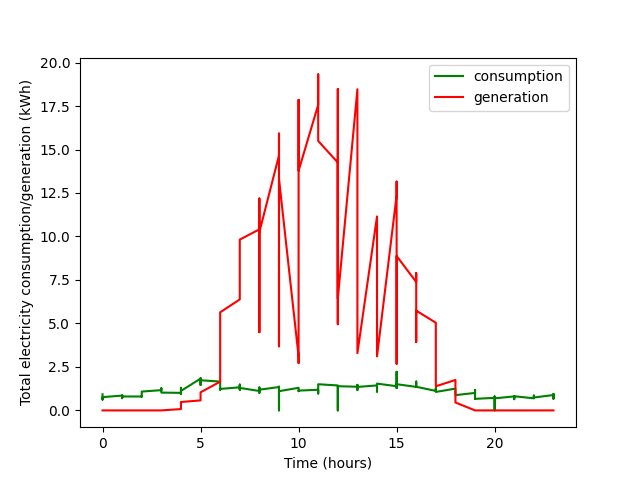
\includegraphics[width=0.5\textwidth]{report/figure/data_collection_1_v1.png}
    \caption{The electricity generation and consumption with the risk of disturbance.}
    \label{fig:1}
\end{figure}

\section{Reinforcement learning}
The mathematical context of Markov decision process (MDP) can be considered as a formal framework to formalize diverse RL methods for learning optimum decision-making policies in a fully or partially observable environment. One of the important issues is the intelligent agent can dynamically make decisions based on actions, states, and rewards where the states refer to possible network configurations and reward (or penalty) stands for feedback signal from the network (environment) that implies the agent’s performance. However, traditional RL has distinct two limitations: (1) Difficulty of applicability to the complex environment and (2) Dendepent on the single agent problem. Traditional RL cannot perform well in the complex environment when the agent encounters the state for the first time. This is because MDP-based traditional RL should control and compute the probability of all states within the environment. Moreover, traditional RL only explores the single agent for the simplicity of the model. They only solved the common problem that all agents take the same actions sharing states. However, most of the world does not have the same characteristics in the agents corresponding to a state. Overall, recent researchers have solved this problem by using deep neural network and multi-agent concepts. 

\subsection{A2C MARL}
Multi-agent reinforcement learning studies how multiple agents interact in a common environment. That is, when these agents interact with the environment and one another, can we observe them collaborate, coordinate, compete, or collectively learn to accomplish a particular task. Independent synchronous Advantage Actor-Critic (IA2C) is a variant of the commonly used A2C algorithm for decentralized training in multi-agent systems. Each agent has its own actor to approximate the policy and critic network to approximate the value function. Both actor and critic are trained, and conditioned on the history of local observations, actions, and rewards the agent perceives, to minimize the A2C loss. 

\subsection{Algorithm}
Multi-agents represent the prosumer, an individual who is both consumes and produces, producer, and consumer. They take three actions the role of battery, and pairs of emergency responses (generation, consumption). The role of the battery ($a_1$) includes that trading the surpluses and shortages of electricity with an external network, charging batteries by the surplus of electricity production, discharging the battery when consumption is greater than production to compensate required energy. In more detail, to take action of the role of battery among three action probabilities, Firstly, we computed the current battery state (CBS) using \textbf{Eq. \eqref{eq_111}}
\begin{equation} \label{eq_111}
    CBS = PBS + (a_1 - 3 ) * (a_1 - 4) * Surp
\end{equation}
where PBS is previous battery state and Surp denotes the surplus electricity. Furthermore, through three actions, we calculate the reward function with seven reward factors: reward for charging the battery, reward for charging the battery with selling the surplus energy, reward for discharging the battery, reward for selling the surplus energy with selling price, reward for buying energy from the grid, reward for the emergency responded in PV, and reward for the emergency responded in load. For example, in the reward for charging the battery, when the agent charges the battery too much, we give the penalty to prevent the charging values over battery capacity. Overall, the reward function can be computed by summing these reward factors.
Finally, carbon dioxide (CO$_2$) emission can be computed by multiplying surplus energy with 03855535 (conversion of energy shortfall (kWh) into emitted CO$_2$ (kg). 

\section{Result}
This project tested the developed algorithm with re-implementing the algorithm (\cite{b4}) to detect the risk of disturbances in generation and consumption and to mitigate this emergence in the energy training on the microgrid concept. \textbf{Fig. \ref{fig2} and \ref{fig3}} displayed the convergence curves of the 1000-episode moving of the episodic total reward in the distribution network for the two different MARL algorithms. 
\begin{figure}[htp]
\begin{subfigure}{0.45\columnwidth}
  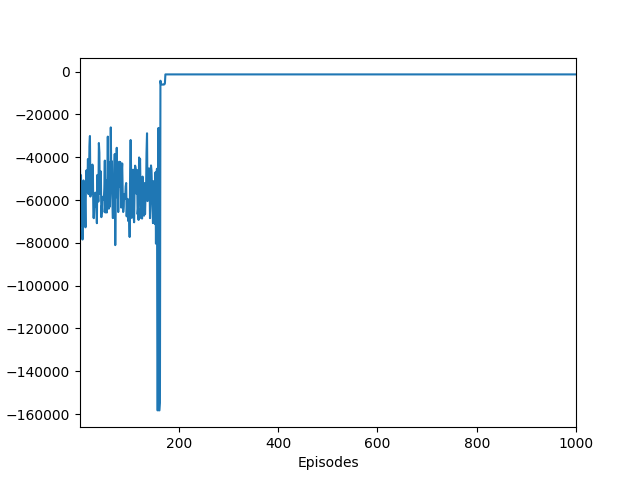
\includegraphics[width=\textwidth]{report/figure/result_1_v1.png}
  \caption{Learning graph via reward in first agent}
  \label{fig2}
\end{subfigure}
\hfill
\begin{subfigure}{0.45\columnwidth}
  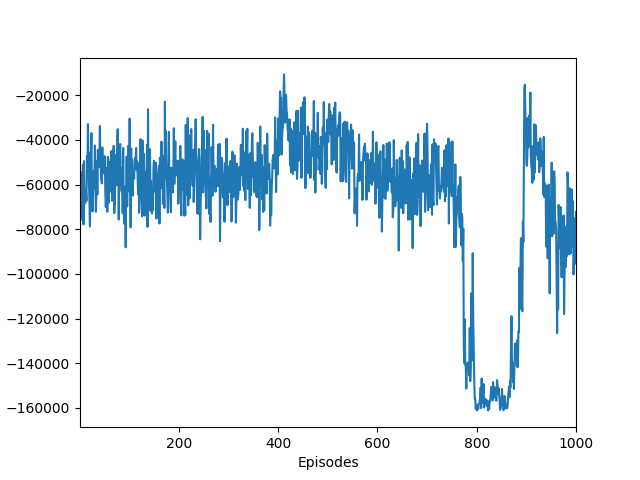
\includegraphics[width=\textwidth]{report/figure/result_1_v2.png}
  \caption{Learning graph via reward in second agent}
  \label{fig3}
\end{subfigure}
\end{figure}
It is evident that the first agent's episodic total reward can be converged in around 200 episodes. On the other hand, the second agent's episodic total reward cannot be converged in whole episodes, in addition, to the catastrophic problem after around 800 episodes. It implies that the learning model abruptly forgets previously learned information upon learning new information and falls into the local minima solution. 

Additionally, \textbf{Fig. \ref{fig4} and \ref{fig5}} shows the evaluation of detection success whether the model can take correct actions (emergency response) corresponding to the ground truth (actual emergence class: 1. night, 2. daytime, 3. peak time, 4. emergency). 
\begin{figure}[htp]
\begin{subfigure}{0.45\columnwidth}
  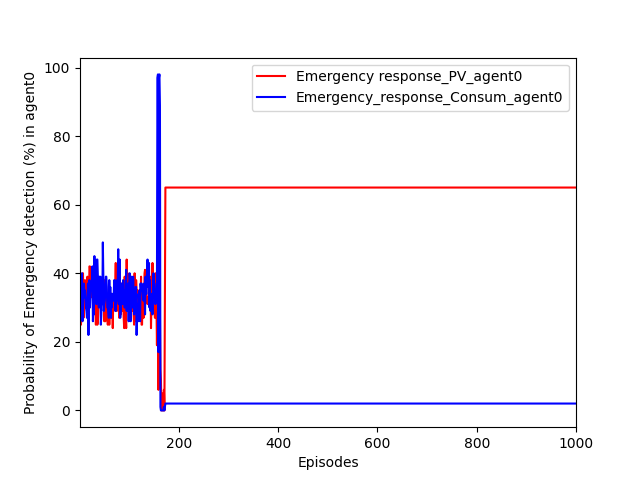
\includegraphics[width=\textwidth]{report/figure/result_2_v1.png}
  \caption{The evaluation of detection success for PV and load in first agent}
  \label{fig4}
\end{subfigure}
\hfill
\begin{subfigure}{0.45\columnwidth}
  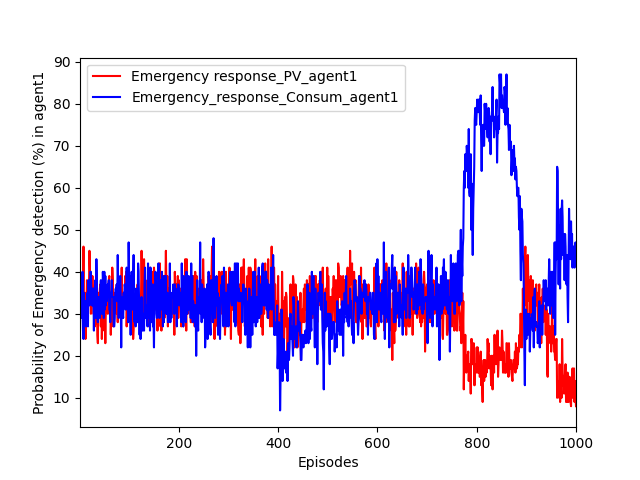
\includegraphics[width=\textwidth]{report/figure/result_2_v2.png}
  \caption{The evaluation of detection success for PV and load in second agent}
  \label{fig5}
\end{subfigure}
\end{figure}
The red lines represent the accuracy of detection success for PV in first agent and second agent and the blue lines represent the accuracy of detection success for load in first agent and second agent. The results showed that the two agents got similar accuracy about around 40\% until the convergence in first agent and catastrophic problem in second agent. Specifically, the first agent has distinct patterns after convergence points that the accuracy of emergency response in PV is higher than in consumption. On the other hand, the second agent has opposite patterns with first agent that the accuracy of emergency response in consumption is higher than in generation. It implies that there are subsequent relationship between generation and consumption in emergency response. 

To further analysis of our model, we showed how the model can mitigate load disturbance in energy trading. it is represented by battery capacity (kW). Both of results \textbf{Fig. \ref{fig6} and \ref{fig7}}showed that the mitigation of energy trading occurs in the load disturbance.

\begin{figure}[htp]
\begin{subfigure}{0.45\columnwidth}
  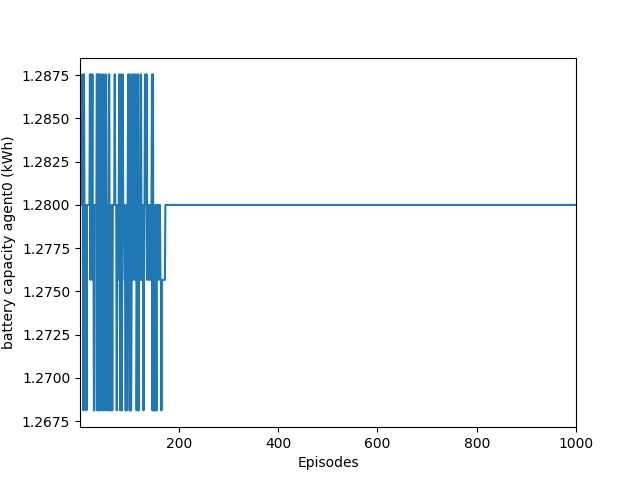
\includegraphics[width=\textwidth]{report/figure/result_3_v1_2.png}
  \caption{The mitigation of emergency situation on the energy trading (battery capacity) in first agent}
  \label{fig6}
\end{subfigure}
\hfill
\begin{subfigure}{0.45\columnwidth}
  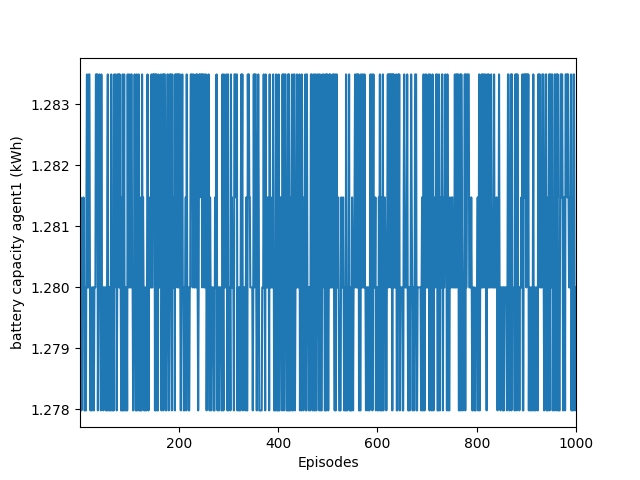
\includegraphics[width=\textwidth]{report/figure/result_3_v2.png}
  \caption{The mitigation of emergency situation on the energy trading (battery capacity) in second agent}
  \label{fig7}
\end{subfigure}
\end{figure}

The results showed that the range of battery capacity can be formed 1.2675 (kW) to 1.2875 (kW) in the first agent until convergence points and 1.278 (kW) to 1.283 (kW) in the second agent until the catastrophic problem. The reason for the tiny gap between maximum and minimum capacity may be related with the data time resolution. Our data time resolution is 5 minutes that cannot be substantial consumption or generation between 5-minute laps. These ranges are dramatically reduced in the occurrence of emergency situations. It implies that the model can sufficiently mitigate the dramatic energy changes by emergency disturbances and have a stable learning with mitigation. This stable pattern disappears after convergence in the first agent and the catastrophic problem in the section agent. 

Finally, the reduction of CO$_2$ emissions through surplus electricity is a constant as 0.1243 (kg).

\section{Discussion \& Conclusion}
This project developed the microgrid energy trading model with mitigating emergency disturbance using deep reinforcement learning. Proposed method tried to detect the emergency events while estimating the energy trading with maximizing the reduction of CO$_2$ emissions. However, the proposed method can stably learn the energy trading rule well but has low performance in detecting emergency situation. There are two reasons (1) low quality of datasets and (2) deficiency of extracting features in the environment. One of reason for this problem may be caused by the low quality of the dataset. We split one dataset, computed by one simulation, into two sets for two agents. Two agents shared similar information patterns and it may result in poor learning performance. Moreover, our model built up with a deep neural network (i.e., a fully connected model) cannot capture sufficient features on the numerical state from the dataset. General DER or Microgrid datasets are graph-structured format that involves the relationship between agents, and energy trading networks with hidden features. However, time series-based table-shaped datasets did not include this relationship and network features, and thus, model cannot explore the relationship and energy trading patterns.

This model can contribute to building microgrid-based resilience enhancement. It can also contribute to reducing the risk of disturbance in the energy trading. In the future, we will develop the current model with building it on meta-learning and graph neural network. 


\begin{thebibliography}{00}
\bibitem{b1} Marqusee, J., Becker, W., and Ericson, S. (2021).  ``Resilience and economics of microgrids with PV, battery storage, and networked diesel generators,'' Advances in Applied Energy, 3, 100049.
\bibitem{b2} Hamidieh, M., and Ghassemi, M. (2022). Microgrids and resilience: A review. IEEE Access, 10, 106059-106080.
\bibitem{b3} Rezazadeh, F., and Bartzoudis, N. (2022, November). A federated DRL approach for smart micro-grid energy control with distributed energy resources. In 2022 IEEE 27th International Workshop on Computer Aided Modeling and Design of Communication Links and Networks (CAMAD) (pp. 108-114). IEEE.
\bibitem{b4} Feng, C., and Liu, A. L. (2024). Networked Multiagent Reinforcement Learning for Peer-to-Peer Energy Trading. arXiv preprint arXiv:2401.13947.
\bibitem{b5} ELamin, M., Elhassan, F., and Manzoul, M. A. (2021, February). Comparison of deep reinforcement learning algorithms in enhancing energy trading in microgrids. In 2020 International Conference on Computer, Control, Electrical, and Electronics Engineering (ICCCEEE) (pp. 1-6). IEEE.
\bibitem{b6} U.S. Billion-Dollar Weather and Climate Disasters 1980—Present, May 2020, [online] Available: https://accession.nodc.noaa.gov/0209268.
\bibitem{b7} Wang, Z., and Wang, J. (2015). Self-healing resilient distribution systems based on sectionalization into microgrids. IEEE Transactions on Power Systems, 30(6), 3139-3149.
\bibitem{b8} Popovic, Z. N., Knezevic, S. D., and Brbaklic, B. S. (2020). A risk management procedure for island partitioning of automated radial distribution networks with distributed generators. IEEE Transactions on Power Systems, 35(5), 3895-3905.
\bibitem{b9} Sharma, A., Srinivasan, D., and Trivedi, A. (2016). A decentralized multi-agent approach for service restoration in uncertain environment. IEEE Transactions on Smart Grid, 9(4), 3394-3405.
\bibitem{b10} Biswas, S., Singh, M. K., and Centeno, V. A. (2021). Chance-constrained optimal distribution network partitioning to enhance power grid resilience. Ieee Access, 9, 42169-42181.
\bibitem{b11} S. A. Arefifar, Y. A.-R. I. Mohamed and T. H. El-Fouly, "Supply-adequacy-based optimal construction of microgrids in smart distribution systems", IEEE Trans. Smart Grid, vol. 3, no. 3, pp. 1491-1502, Sep. 2012.
\bibitem{b12} T. Ding, Z. Wang, W. Jia, B. Chen, C. Chen and M. Shahidehpour, "Multiperiod distribution system restoration with routing repair crews mobile electric vehicles and soft-open-point networked microgrids", IEEE Trans. Smart Grid, vol. 11, no. 6, pp. 4795-4808, Nov. 2020.
\bibitem{b13} K. S. Fuad, H. Hafezi, K. Kauhaniemi and H. Laaksonen, "Soft open point in distribution networks", IEEE Access, vol. 8, pp. 210550-210565, 2020.
\bibitem{b14}  X. Jiang, Y. Zhou, W. Ming, P. Yang and J. Wu, "An overview of soft open points in electricity distribution networks", IEEE Trans. Smart Grid, vol. 13, no. 3, pp. 1899-1910, May 2022.
\bibitem{b15} M. Barani, J. Aghaei, M. A. Akbari, T. Niknam, H. Farahmand and M. Korpas, "Optimal partitioning of smart distribution systems into supply-sufficient microgrids", IEEE Trans. Smart Grid, vol. 10, no. 3, pp. 2523-2533, May 2019.
\bibitem{b16} C. Chen, J. Wang, F. Qiu and D. Zhao, "Resilient distribution system by microgrids formation after natural disasters", IEEE Trans. Smart Grid, vol. 7, no. 2, pp. 958-966, Mar. 2016.
\bibitem{b17} T. Ding, Y. Lin, G. Li and Z. Bie, "A new model for resilient distribution systems by microgrids formation", IEEE Trans. Power Syst., vol. 32, no. 5, pp. 4145-4147, Sep. 2017.
\bibitem{b18} H. Qi, X. Wang, L. M. Tolbert, F. Li, F. Z. Peng, P. Ning, et al., "A resilient real-time system design for a secure and reconfigurable power grid", IEEE Trans. Smart Grid, vol. 2, no. 4, pp. 770-781, Dec. 2011.
\bibitem{b19} Papoudakis, G., Christianos, F., Schäfer, L., and Albrecht, S. V. (2020). Benchmarking multi-agent deep reinforcement learning algorithms in cooperative tasks. arXiv preprint arXiv:2006.07869.


\end{thebibliography}

\end{document}
